\section{Serving measurements}\label{sec:serving}

How fast the scorer's server generates tokens decides how many model calls an agent can afford per task, and whether
more than one agent can work on a task at the same time. We measured it before designing any agent.

\paragraph{Method.} A Kaggle notebook with four L4 GPUs started the vLLM server with the flags of the starter notebook
\citep{holbrook2026starter}: the model split over the four GPUs, a maximum context of 32,768 tokens, and the Gemma 4
parsers. A client then sent streaming completion requests with prompts of random tokens. For each prompt length and
each number of concurrent streams, a first request generated one token, which measures the processing of the prompt
(prefill) and fills the prefix cache; a second request with the same prompt generated 160 tokens, which measures
decoding on a cached prefix. The 31B, 12B and E4B models were measured one after another, each with its own server.
A second session repeated the 31B measurement with a LoRA adapter loaded. The \ServeRows{} measured cells and the
server records are in \texttt{serving\_bench.csv} and \texttt{serving\_servers.csv}.

\begin{table}[t]
\centering
\small
\caption{Serving throughput on four L4 GPUs (vLLM, one server per model). Context: prompt tokens already in the request. Streams: concurrent requests. Each request generates 160 tokens.}
\label{tab:serving}
\begin{tabular}{lrrrrr}
\toprule
Model & Context & Streams & Prefill tok/s & Decode tok/s per stream & Decode tok/s, all streams \\
\midrule
31B & 2{,}048 & 1 & 1{,}539 & 38.1 & 38 \\
31B & 2{,}048 & 2 & 1{,}545 & 34.4 & 66 \\
31B & 2{,}048 & 4 & 1{,}546 & 31.2 & 122 \\
31B & 2{,}048 & 8 & 1{,}550 & 17.9 & 78 \\
31B & 2{,}048 & 16 & 1{,}548 & 18.2 & 279 \\
31B & 8{,}192 & 1 & 1{,}479 & 36.3 & 36 \\
31B & 8{,}192 & 2 & 1{,}480 & 33.7 & 66 \\
31B & 8{,}192 & 4 & 1{,}485 & 29.3 & 114 \\
31B & 8{,}192 & 8 & 1{,}486 & 9.2 & 25 \\
31B & 14{,}336 & 1 & 1{,}426 & 35.5 & 35 \\
31B & 14{,}336 & 2 & 1{,}427 & 32.8 & 64 \\
31B & 14{,}336 & 4 & 1{,}429 & 27.9 & 107 \\
\addlinespace
12B & 2{,}048 & 1 & 3{,}054 & 76.1 & 75 \\
12B & 2{,}048 & 4 & 3{,}076 & 60.6 & 235 \\
12B & 2{,}048 & 8 & 3{,}089 & 48.9 & 379 \\
12B & 2{,}048 & 16 & 3{,}082 & 34.6 & 534 \\
12B & 8{,}192 & 1 & 2{,}973 & 69.8 & 69 \\
12B & 8{,}192 & 2 & 2{,}994 & 63.2 & 123 \\
12B & 8{,}192 & 4 & 3{,}002 & 55.0 & 213 \\
\addlinespace
E4B & 2{,}048 & 1 & 5{,}267 & 105.8 & 104 \\
E4B & 2{,}048 & 4 & 5{,}385 & 85.8 & 329 \\
E4B & 2{,}048 & 8 & 5{,}372 & 75.9 & 578 \\
E4B & 2{,}048 & 16 & 5{,}404 & 57.4 & 858 \\
E4B & 8{,}192 & 1 & 5{,}212 & 95.9 & 94 \\
E4B & 8{,}192 & 2 & 5{,}235 & 85.0 & 164 \\
E4B & 8{,}192 & 4 & 5{,}254 & 73.5 & 282 \\
\bottomrule
\end{tabular}
\end{table}


\begin{figure}[t]
\centering
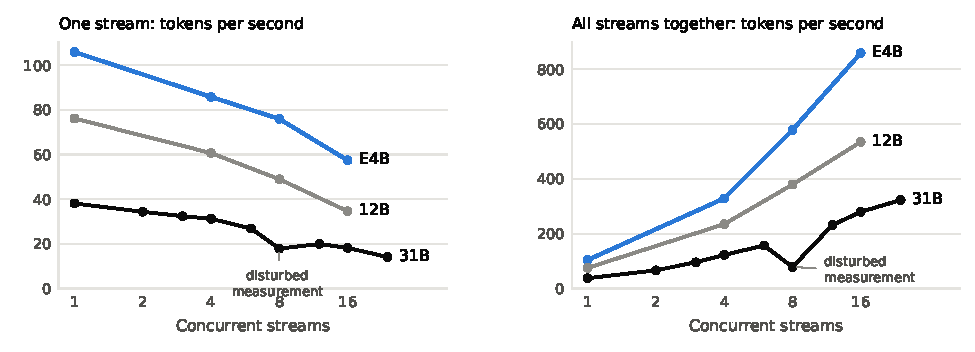
\includegraphics[width=\linewidth]{fig/serving.pdf}
\caption{Decode throughput on four L4 GPUs with a context of 2,048 tokens. Left: tokens per second of one stream as
the number of concurrent streams grows. Right: tokens per second summed over the streams.}
\label{fig:serving}
\end{figure}

\paragraph{One stream.} The 31B model decodes \ServeBigOne{} tokens per second with a short context and
\ServeBigLong{} with 14,336 tokens of context (\cref{tab:serving}). The 12B model reaches \ServeMidOne{} and E4B
\ServeSmallOne{} tokens per second, \ServeRatioSmallBig{} times the 31B model. Prefill is fast in comparison: about
\ServeBigPrefill{} tokens per second for 31B. An agent that keeps its prompt prefix stable pays this once, because the
server reuses cached prefixes. Generated tokens are what costs time: a 31B call that writes 1,000 tokens takes about
half a minute. The server needs \ServeBigStartup{}~s to start with the 31B model, which counts against the time limit
of a scoring run.

\paragraph{Several streams.} Concurrent streams share the GPUs (\cref{fig:serving}). With four streams and a long
context, each 31B stream still decodes \ServeBigFourPer{} tokens per second, \ServeBigFourAgg{} in total. Apart
from one cell discussed below, the total grows up to 16 streams for all three models, to \ServeBigSixteenAgg{} tokens per second for 31B and
\ServeSmallSixteenAgg{} for E4B at 2,048 tokens of context. The scorer runs tasks one after another, so this capacity
is only useful to an agent that runs several model calls in parallel within one task.

\paragraph{Two cells that do not fit.} With eight streams of 8,192 tokens, the 31B server delivered 9.2 tokens per
second per stream, a third of the four-stream value. The server reported a key-value cache of \ServeBigKV{} tokens
for 31B, against \ServeMidKV{} for 12B and \ServeSmallKV{} for E4B, and eight contexts of 8,192 tokens hold 65,536
tokens. We read the drop as cached prefixes being evicted and processed again; we did not test this reading. With
eight streams of 2,048 tokens the 31B server gave 17.9 tokens per second per stream and 78 in total, less in total
than with four streams (122) and with 16 (\ServeBigSixteenAgg). We have no explanation for this cell and report it as measured;
\cref{fig:serving} marks it.

\begin{table}[t]
\centering
\small
\caption{Cost of serving a LoRA adapter with the 31B model (same server settings; requests addressed to the adapter). Decode speed in tokens per second per stream; change against the control in brackets.}
\label{tab:adapter}
\begin{tabular}{lrrrr}
\toprule
Server & KV cache, tokens & 2k context, 1 stream & 8k, 1 stream & 8k, 4 streams \\
\midrule
no adapter (control) & 46{,}352 & 38.3 & 36.4 & 29.4 \\
rank 16, attention projections & 37{,}328 & 33.9 (\ensuremath{-}12\%) & 32.4 (\ensuremath{-}11\%) & 26.9 (\ensuremath{-}9\%) \\
rank 16, all linear layers & 37{,}328 & 33.8 (\ensuremath{-}12\%) & 32.5 (\ensuremath{-}11\%) & 26.9 (\ensuremath{-}9\%) \\
rank 8, two module types & 37{,}568 & 33.3 (\ensuremath{-}13\%) & 32.1 (\ensuremath{-}12\%) & 26.7 (\ensuremath{-}9\%) \\
\bottomrule
\end{tabular}
\end{table}


\paragraph{Cost of an adapter.} The competition allows LoRA adapters on the one served model. With an adapter of rank
16 or rank 8 loaded, requests addressed to the adapter decoded \AdapterLossMin{} to \AdapterLossMax\% slower than
requests to the same server without an adapter (\cref{tab:adapter}), and the reported key-value cache shrank by
\AdapterKVLoss\% to \AdapterKV{} tokens. Requests addressed to the base model on a server with a loaded adapter
changed by \AdapterBaseMin{} to \AdapterBaseMax\% (one stream, short context). Which layers the adapter covers made no visible difference. The
measurements were made once per cell.

\paragraph{What followed for the design.} At 35 tokens per second, an agent with a limit of eight minutes per task,
the limit of the public configuration \arm{BF5}, can generate at most about 17,000 tokens, before the time of its tool
calls and of prefill is taken off. A second agent that works in parallel
slows the first by about a tenth at two streams. E4B generates \ServeRatioSmallBig{} times as fast, so the same task
limit is rarely what stops an E4B agent (\cref{sec:cost}).
